\documentclass[10pt,a4paper]{article}
 \usepackage[utf8]{inputenc}
 \usepackage{helvet}
 \renewcommand{\familydefault}{\sfdefault}
 \usepackage{graphicx}
 \usepackage{verbatim}
 \usepackage[english]{babel}
 \usepackage{babelbib}
 \graphicspath{{Images/}}
 \usepackage{fancyhdr}
 \usepackage{url}

\pagestyle{fancy}
\rhead{Multiplayer game design, Vili Lipo, 014814253}
\selectbiblanguage{english}
 \author{Vili Lipo, 014814253}
 \title{Multiplayer Game Design}

 \begin{document}
 \maketitle
 \thispagestyle{plain}
 \section{Introduction}

 This design document is for a multi-player two-dimensional space shooter
 death-match that is playable up to 16 players.  Figure 1 represents what the
 game could look like, it shows ships, their health-bars, some bullets and a
 space rock.  With 16 players the gaming experience stays enjoyable. Beyond
 that game becomes confusing and other problems like spawn killing start to
 degrade the experience. Scaling the game beyond this would mean running
 multiple concurrent matches. For concurrent matches, multiple processes is
 used as servers for the distinct matches do not have any particular reason
 to share information between each other.
 
 The game server will use event based I/O-multiplexing to ensure quick response
 times to user actions. In addition to this common error compensation
 techniques are used to make the experience more pleasant.

 In this system both the server and the clients simulate the game state. If the
 simulations differ the server state rules over the client states.  This is
 called  client-side prediction and server reconciliation~\cite{gambetta_fast}.
 This is the common hierarchy, as doing the hierarchy other way enables
 cheating.

 Reliability of the system is enforced with constant state updates between the
 clients and the server. The game state is sent 20 times in a second from the
 server to the clients, so if individual packet loss happens it's effects are
 mitigated in under a second. This can use a lot of bandwidth and cause
 congestion in the network, but it benefits the responsiveness and reliability
 of the server.

 No error recovery is used as the data sent between clients and the server is
 highly time sensitive, and recovered packages would probably lose their
 relevancy during an extra round-trip time. Error correction could maybe be
 used, but the overhead might hinder responsiveness of the game and use more
 bandwidth. For these reasons, reliability of this game is based only on the
 constant state updates and error compensation.

 Clients can load for the game that change the look and feel of
 the ship and the map background. These downloads use different mechanisms than
 the game-play networking. The resources are served with regular TCP file
 transfer methods. The loaded assets are validated using checksums.

 The design does not assume that the clients can connect to each other
 because of the strict NAT-types, but it the server must be able to 
 receive and send UDP-traffic to all participants. So NAT and Firewall settings
 for the server side must be configured correctly.

 \begin{figure}
   \caption{Concept art for the game}
   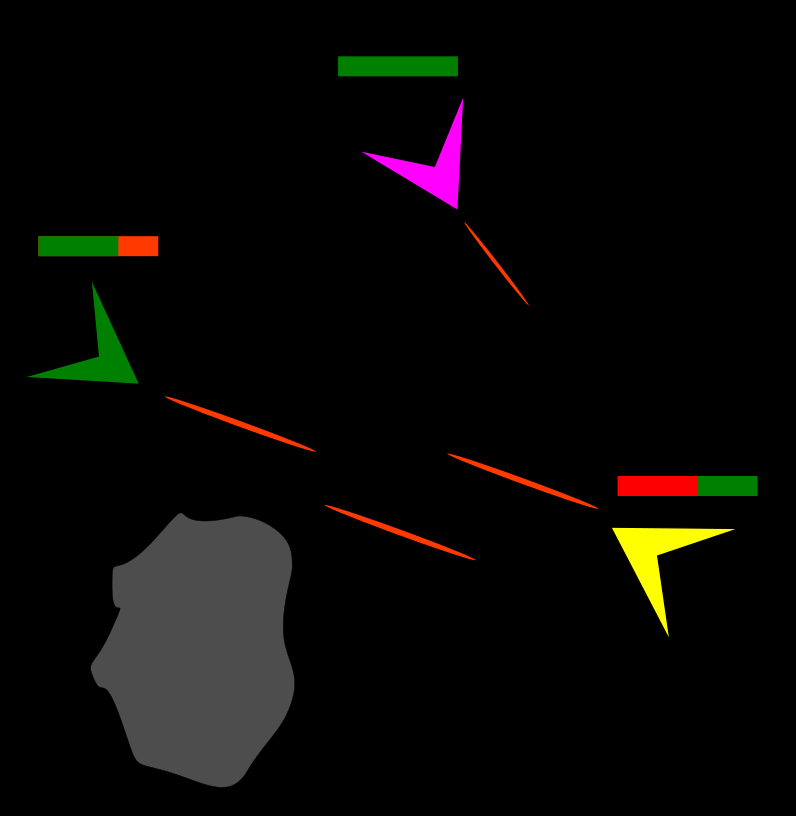
\includegraphics[scale=0.4]{concept.png}
 \end{figure}

 \section{Game logic and engine}

 The game consists of a map, player controlled ships, and bullets.  The map is
 a empty area of space in which the ships can battle out. The map has limited
 size and if a player ship hits the border it will be damaged. The map contains
 a data structure that allows it to check for collisions in near constant time.

 The player ships have 10 hit-points. One hit-point is subtracted every time
 the ship receives damage. The goal of the players is to destroy as many other
 players as possible.  Players can damage opponents ships by shooting bullets.
 The ship data model contains information about their hit-points, heading and
 speed.

 The bullets are simple data-objects that spawn when a ship shoots. The bullet
 has static speed and direction, along with location information. This
 allows both the client and the server to simulate bullet movements concurrently.
 Figure 2 displays simple domain model of the game logic.
 
 The map object contains a hash-map data-structure in which the each key represents
 a map dot on the map that contains something. If some key contains two values
 it is a collision and then the damage calculation is preformed on the object.

 The game engine aims to constantly run the game at 60 game cycles per seconds
 and it updates the state to server 20 times per second. A game cycle contains
 of the following actions; apply server state every third cycle, register user input, check
 collisions, calculate hit points and send a input to the server.

 \begin{figure}
   \caption{Simple model of the game logic}
   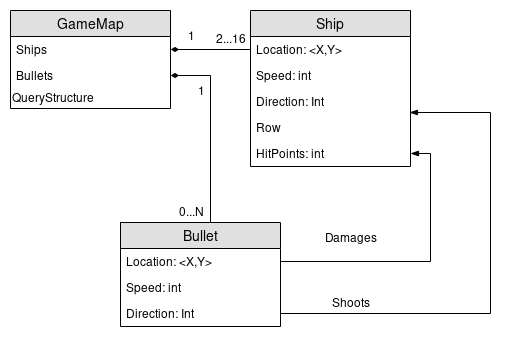
\includegraphics[scale=0.6]{simpleModel.png}
 \end{figure}

 \section{Client-server communications}

 In this application clients and the server communicate with each other trough
 UDP. UDP is preferred TCP because this application is very time sensitive.  In
 this domain it is better to just lose packets than try to retransmit. The
 retransmitted packages will be already out of date when they are finally
 received, hence retransmitting only furthers network congestion.

 With UDP reliability must be implemented at application level. In this
 application the client and server game engines try to simulate the game state
 as best they can with the information at hand. This helps with small amounts
 of sporadic packet loss, but this practice is weak against error bursts. 

 The game state is transferred between the client and the server in JSON-format
 that follow the description of the message frame shown in figure 3.  The
 message frame contains a small header for transmitting necessary information
 that is not obvious from the game state on its own.  


 Client ID is used to identify the client.
 Cycle ID is used mostly for debugging purposes. It 
 can be used to determine if client or server software start
 to miss tick-time deadlines.

 Time-stamp is used in entity interpolation.  When a client sees other ships in
 the game those are actually the other ships from the previous tick-time.
 Time-stamp is also used to lag-compensate hit detection at the server.  The
 lag is caused by the entity interpolation, so effectively every client sees
 the other ships 50ms in the past. With a time-stamp the server can reconstruct
 every client state between ticks and treat them fairly~\cite{bernier_latency}.
 The time-stamp can also be used to calculate latency between the client and
 the server. The latency figure can be used to make the lag compensation even
 more accurate.  If the game would be expanded to host multiple concurrent
 matches a match identifier field is added to the header.

The game information contains the game state of the past 3 ticks. The client
needs these for entity interpolation. The client sends its input information
to the server 20 times a second. As it is intended that the clients run at 60 cycles
per second it sends the input information for all the cycles. This is visualised in 
figure 4.
 
 \begin{figure}
   \caption{Visualisation of server-to-client message frame}
   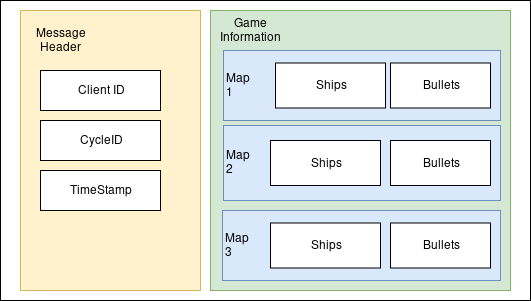
\includegraphics[scale=0.7]{serverMessageFrame.png}
 \end{figure}

 \begin{figure}
   \caption{Visualisation of client-to-server message frame}
   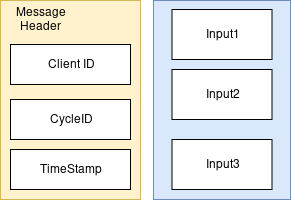
\includegraphics[scale=0.7]{clientMessageFrame.png}
 \end{figure}

 Network error burst will cause something that gamers usually refer as a `lag
 spike', in which the controls issued by the player do not get the desired
 outputs. When the client states are synced with the server state after a burst
 of packet loss players will experience phenomena usually called
 `rubber-banding', in which the player ships are moved to a location correct in
 the servers point of view. This makes the game less enjoyable, but keeping the
 client state as the correct state would open a huge can of worms when it comes
 to cheating possibilities. 

 The client joins the match hosted by the server using a special handshake message.
 When this message arrives at the server the client is added to the match, if
 there is still room in the 16 player quota. The client has knowledge of 
 some servers and can try to connect to every one of them.


\section{Server architecture}

The server will follow event driven architecture. There is two kinds of events
in this application, the messages coming from the clients and the tick-timer of the server.

Event handler for client messages applies the changes of the client state to the
server state if those follow the game rules. 
Event handler for tick-timer will send the server state to all clients.  
Performance of the server is dependent on calling non-blocking I/O-calls especially
for the sending the state to the clients.

So to implement this design the programming environment needs to support
asynchronous I/O and event loops. Despite this the server responsiveness will
slow down as player count increases. To meet the goal of 20 updates per second,
the server will have to validate the 16 player game states and send the correct
game state back to the clients within 0.05 seconds. That leaves 3.15
milliseconds to validate player game state, assuming that those arrive on time.
These strict time limitations make it appealing to run concurrent matches in
separate processes, given that the host system has the network resources to
handle multiple matches.

In this system there is an additional micro-service that only keeps track
of the online-game-servers and gives this list to the clients. From this 
list the client can see the player count and ping of each server.
The server has a component that sends its information to the game-list-server,
containing name, ip-address, and player count.

\section{Downloading game settings}

The clients can download new assets to the game, from a separate asset server
that uses TCP-for transferring the assets to the client.

The assets contain but are not limited to new ship designs, new background textures and
different ambient music tracks. The user can select assets through a settings menu.

The client source code
contains MD5-checksums for all available assets, that are used for end-to-end
error detection and recovery. If the checksum does not match with the one calculated
from the received data the user is prompted and the client retries the download.

\newpage
\bibliographystyle{babplain-lf}
\bibliography{sources}


 
 \end{document}

